\documentclass[12pt]{article}

\usepackage{fullpage}
\usepackage{amsmath}
\usepackage{epsfig}
\usepackage{graphics}
\usepackage{caption}

\usepackage{hyperref}
\hypersetup{
    colorlinks=true,
    linkcolor=blue,
    filecolor=magenta,
    urlcolor=cyan,
  }

\usepackage{parskip}

\usepackage{mdframed}
\newenvironment{graybox}%
  {\begin{mdframed}[backgroundcolor=lightgray]}%
  {\end{mdframed}}

\usepackage[dvipsnames]{xcolor}

\usepackage{enumitem,amssymb}
\newlist{todolist}{itemize}{2}
\setlist[todolist]{label=$\square$}

\oddsidemargin -0.15in
\evensidemargin -0.15in
\headheight 0in
\headsep 0in
%\topmargin -0.25in
\textheight 9.3in
\textwidth 6.8in

\begin{document}

% Title page
\begin{center}

  \vspace{5cm}

  {\LARGE \bf Guide to writing a lab report}

  \vspace{1cm}

  {\Large Modern Physics (PHY 223)}

  \vspace{10cm}

  {\Large Franklin \& Marshall College}

  \vspace{1cm}

  {\Large Last updated: \today}

\end{center}

\newpage

\hypertarget{contents}{}
% Print table of content
\tableofcontents

\newpage

\section{Overview}

This document is intended to be used as a reference while you write
your lab report. We recommend you use the pre-writing (Sec.~\ref{sec:pre-chk}) 
and post-writing (Sec.~\ref{sec:post-chk})
checklists to improve the process of writing the report and the
quality of your manuscript. In Sec.~\ref{sec:order}, we propose an
order to writing the various sections of your manuscript. Before
writing any parts of your report, review the relevant instructions in 
Sec.~\ref{sec:whattowrite} as linked
 in the Table of Contents on the previous page.
% (sections \ref{sec:Abstract}, \ref{sec:Introduction},
% \ref{sec:Theory}, \ref{sec:Methods}, \ref{sec:Data},
% \ref{sec:Conclusion}, \ref{sec:Acknowledgments}, and
% \ref{sec:References}).
More information about the appropriate styles for figures and tables are given
in Sec.~\ref{sec:style}.

\newpage

\section{Checklist: Before you write}
\label{sec:pre-chk}

\vspace{3mm}


\begin{todolist}

\item {\bf Review the literature}. You should research your topic
  thoroughly.  This can be done as you are taking and analyzing data.

\item Finish taking your {\bf data}.

\item {\bf Create an initial set of figures} for your report.

\item {\bf Complete your analysis} of the results. This should include full
consideration of uncertainty.

\item Based on your results, {\bf write down your claim}. This should
  be the answer to a well-formed question. When possible, your claim
  should include numbers.

\vspace{2mm}

\noindent Example of a bad claim:

\begin{em}
  As the temperature of the heat reservoir changed, so did the temperature of
  the metal cylinder attached to it.
\end{em}

\vspace{2mm}

\noindent Example of a better claim:

\begin{em}
  We measure a heat transfer coefficient of (10.3 $\pm$ 0.4) W/(m$^{2}$.K)
  between the heat reservoir and the metal cylinder.
\end{em}

\item {\bf Revise your figures} based on your claim. Do the figures present the
  right supporting information? Are all the figures relevant to the narrative?

\item Think about your {\bf target audience.} Consider the level of knowledge
of the people you are writing for.

\end{todolist}

\newpage

\section{Steps to write a report or article}
\label{sec:order}

Reports and articles do not have to be written beginning to end. In
fact, writing an introduction or an abstract should be impossible
until many other components are present in the text. While there is no
``one-size-fits-all'' method, consider the steps below as a good
starting point:

\begin{enumerate}
\item Prepare the figures and data tables. Upload them first into your
  report. Create informative captions for each of them.

\item Write the experimental/computational methods section.

\item Write your results and analysis. These can be in different
  sections or joined together.

\item Write your conclusion.

\item Write your theory section. Based on your analysis, figure out
  what math and physics you need to cover to bring your target
  audience to an understanding of the claim. You don't have to spell
  everything out.  You can refer other texts for lengthier
  derivations.

\item Write your introduction. Now that you have the full story, you
  can create an introduction that offers a starting point for your
  narrative.

\item Write the abstract.

\end{enumerate}

No matter the order in which you write the report, you will have to
iterate through the writing process. You should never consider a
section ``done'' until the whole report is written and is coherent.

You may also consider creating an outline of your manuscript before
you start writing (either the whole report or for individual parts).

\newpage

\section{What to write in a report or article}
\label{sec:whattowrite}

In this section, tips, tricks, and examples are given for each
section of a report:

\begin{enumerate}
\item \hyperref[sec:Abstract]{Abstract}
\item \hyperref[sec:Introduction]{Introduction}
\item \hyperref[sec:Theory]{Theory Section}
\item \hyperref[sec:Methods]{Methods}
\item \hyperref[sec:Data]{Data and Analysis}
\item \hyperref[sec:Conclusion]{Conclusion}
\item \hyperref[sec:Acknowledgments]{Acknowledgments}
\item \hyperref[sec:References]{References}
\end{enumerate}

\newpage

\subsection{Abstract}
\label{sec:Abstract}

 An abstract should contain the following information:

 \begin{itemize}
  \item The \textcolor{red}{objective} of report
  \item The \textcolor{violet}{method}
  \item The \textcolor{ForestGreen}{result(s)} including an uncertainty whenever possible.
  \item A short \textcolor{BurntOrange}{discussion} of the meaning of the result
  \item Possible {\bf future direction}
 \end{itemize}

 Below is an example abstract:

 \begin{em}
  \textcolor{red}{We demonstrate a high energy throughput, modular optical
  laser pulse shaping technique for generating tunable, narrowband, terahertz
  radiation from the surface of InAs.} \textcolor{ForestGreen}{We achieve a
  frequency selectivity ($\Delta f / f$) of 0.10 at 1.18 THz and demonstrate
  an energy throughput of up to 98\%} \textcolor{violet}{using two etalons to
  create a sequence of optical pulses.} \textcolor{BurntOrange}{In contrast
  with previously reported schemes, our technique does not rely on
  interferometry or involve diffractive optical elements, making it robust and
  relatively inexpensive to implement.} \textbf{This technique can be expanded
  with additional etalons in order to achieve greater frequency selectivity
  without sacrificing efficiency.} \textcolor{BurntOrange}{Finally, we analyze
  the effects of carrier saturation within the InAs as it contributes to the
  spectral shape of the terahertz radiation and selectivity of this method. }
 \end{em}

 This abstract is missing a statement of uncertainty as this particular claim in this
 particular sub-field of physics does not require one. This is an
 exception.

 \newpage

\subsection{Introduction}
\label{sec:Introduction}

\subsubsection{What to include}

The introduction must answer the following questions:

\begin{itemize}
\item What \textcolor{red}{question} are you addressing?
\item What is the \textcolor{violet}{broader context} for the work
  presented? What has been done before?
\item What is the \textcolor{ForestGreen}{motivation} for the work
  presented?
\end{itemize}

In addition to answering those questions, the introduction should
include:

\begin{itemize}
\item A clear \textcolor{BurntOrange}{statement of what work was done}.
\item A brief description of the {\bf method}.
\item Your results. What is your main \textcolor{Sepia}{claim}?
\end{itemize}

Below is an abbreviated introduction as an example. (It is longer than
what needs to appear in a report.)

\begin{em}
  \textcolor{violet}{The last 20 years have seen the development of
    increasingly more efficient terahertz (THz) generation [CITATIONS]
    and detection [CITATIONS] methods, which have been at the core of
    many new research avenues and technologies. Many physical
    processes in materials science exhibit sensitivity to
    THz-frequency radiation, or occur on timescales comparable to that
    of a THz pulse. Applications of THz technology require efficient
    and effective tools for engineering bright THz sources with
    customizable characteristics. Recent work aimed at applying THz
    technology to security [CITATIONS] and industrial [CITATIONS]
    applications has underscored the need for broadband sources. Other
    applications, however, such as coherent control of vibrational
    modes in molecular samples [CITATIONS], require access to
    narrowband, tunable THz sources.}

  \textcolor{ForestGreen}{Motivated by the extensive availability of
    optical components and alignment techniques in the optical regime,
    most methods for producing THz radiation with the desired temporal
    and spectral characteristics demonstrated to date involve control
    of the generation mechanism rather than shaping of the THz
    radiation itself. Manipulation of both the spatial [CITATIONS] and
    temporal characteristics of the optical laser pulse that drives
    the THz generation allows control of the resulting THz
    radiation. For example, narrowband, tunable sources of THz can be
    achieved by purely temporal shaping of the optical laser to create
    a pulse train [CITATIONS]. This optical pulse train creates a THz
    pulse train with a narrow spectrum whose width and center
    frequency can be controlled by adjusting the number of and timing
    between pulses in the train, respectively.}

  \textcolor{violet}{Several methods for creating customizable optical
    pulse trains have been applied to shaping THz. One such method is
    ...}

  \textcolor{violet}{Various THz generation methods have been explored
    using these pulse shaping for manipulating THz radiation. To date,
    efforts have concentrated on photo-conductive antennas
    [CITATIONS], air plasma [CITATIONS], semiconductor
    heterostructures [CITATIONS], and nonlinear optical processes
    [CITATIONS] as tunable THz sources...} \textcolor{red}{To the best
    of our knowledge, none of the work done on THz spectral shaping
    has used un-biased semiconductor chips as their emitter. Such THz
    emitters have a number of advantages: they can be used with
    non-amplified laser sources, they are relatively low-cost, and
    they lack the need of photo-conductive antennas for supporting
    electronics, further simplifying the setup.}

  \textcolor{BurntOrange}{In this paper, we demonstrate a simple,
    non-interferometric, modular scheme for generating tunable,
    narrowband THz radiation using a highly efficient optical pulse
    shaping technique.} \textbf{We use a series of staggered,
    adjustable etalons to create an optical laser pulse train and
    focus it on the surface of an un-biased InAs chip to generate
    THz. Using a series of etalons permits a modular approach that
    allows the desired degree of narrowing of the spectrum, as well as
    relative suppression of unwanted spectral features, at the cost of
    additional optics.} \textcolor{Sepia}{Using this approach, we
    demonstrate a throughput possibly as high as 98\% with a bandwidth
    selectivity $\Delta f / f = 0.10$ at 1.18 THz.}
  \textcolor{BurntOrange}{For comparison, we also test a similar
    scheme involving a single etalon followed by a Michelson
    interferometer... Finally, we study the contribution of carrier
    saturation effects in InAs, and how this affects the shaping
    capabilities of this modular approach.}
\end{em}

\subsubsection{Additional concerns}

\begin{itemize}
\item While you must introduce your main claim in the introduction, do
  not mix those with your analysis and conclusion.
\item The introduction should start with a more global point of view
  and zoom in on the particulars of your work.
\item You can give a roadmap of your report at the end of the
  introduction.
\end{itemize}

\newpage

\subsection{Theory section}
\label{sec:Theory}

 Depending on the experiment, the theory section can significantly vary in
 length. In pure experimental demonstration, it can be almost absent. In
 reports with a more extensive analysis, the theory section should include
 the information needed to explain the claims, using the data as proof.

 As mentioned above, keep your audience in mind as you write this section.

 The theory section {\bf may include}:

 \begin{itemize}
  \item physical concepts that help explain the results. For example, a
  report about the magnetic properties of nickel should include an brief
  introduction to ferromagnetism.
  \item mathematical concepts important for the analysis. For example, if
  you use Fourier analysis to process your results, a quick description of
  what Fourier analysis is and does must be included.
  \item mathematical derivations important for the analysis. If
  your analysis involves deriving a specific value from the a set of
  measurements related by an equation, that equation must be included and
  explained. Some of the steps of the derivation must be shown.
 \end{itemize}

 The theory section {\bf should not include}:

 \begin{itemize}
  \item data or analysis.
  \item information unrelated to the analysis. It is easy to put too much
  information in the theory section. To avoid that, you may use citations
  to include more in-depth treatment of certain topics. For example, if you
  Fourier transforms in your analysis, you should not include all of the
  Fourier transforms properties in the report. You should only highlight the
  one(s) you use directly.
 \end{itemize}

\newpage

\subsection{Methods}
\label{sec:Methods}
\subsubsection{Experimental methods}

 An experimental description should:

 \begin{itemize}
  \item include a least one schematic of the experiment. Photos of the
  experimental setup are usually not appropriate.
  \item include a \textcolor{red}{direct reference} to the figure in the text.
  \item include \textcolor{violet}{\bf labels} in the experimental
    schematic that are referenced in the caption and/or text.
  \item include a \textcolor{violet}{numbered caption to the figure.}
  \item \textcolor{ForestGreen}{describe the experimental setup in the text}.
  \item \textcolor{BurntOrange}{emphasis on the parts of the
      experiment that affect the results. For example, in most cases,
      we don't need to know the make of the laser, only its
      capabilities. }
  \item include important \textcolor{Sepia}{limitations or concerns}
    of the apparatus.
 \end{itemize}

  Below is an example experimental description:

 \begin{em}
   \textcolor{red}{Figure \ref{Fig: Experimental setup} shows a
     schematic of the experimental setup.} \textcolor{ForestGreen}{The
     THz generation is driven by a ~50 fs pulse from a Ti:Sapphire
     laser oscillator with center wavelength 800 nm, pulse energy
     $\sim$8 nJ, and repetition rate 80 MHz. A beam splitter sends 4\%
     of the incident pulse energy to be used for electro-optic
     detection of the shaped THz. The remainder of the power goes
     through the pulse shaping setup before being focused on a InAs
     chip for THz generation.}

 \begin{minipage}{\linewidth}
  \centering
  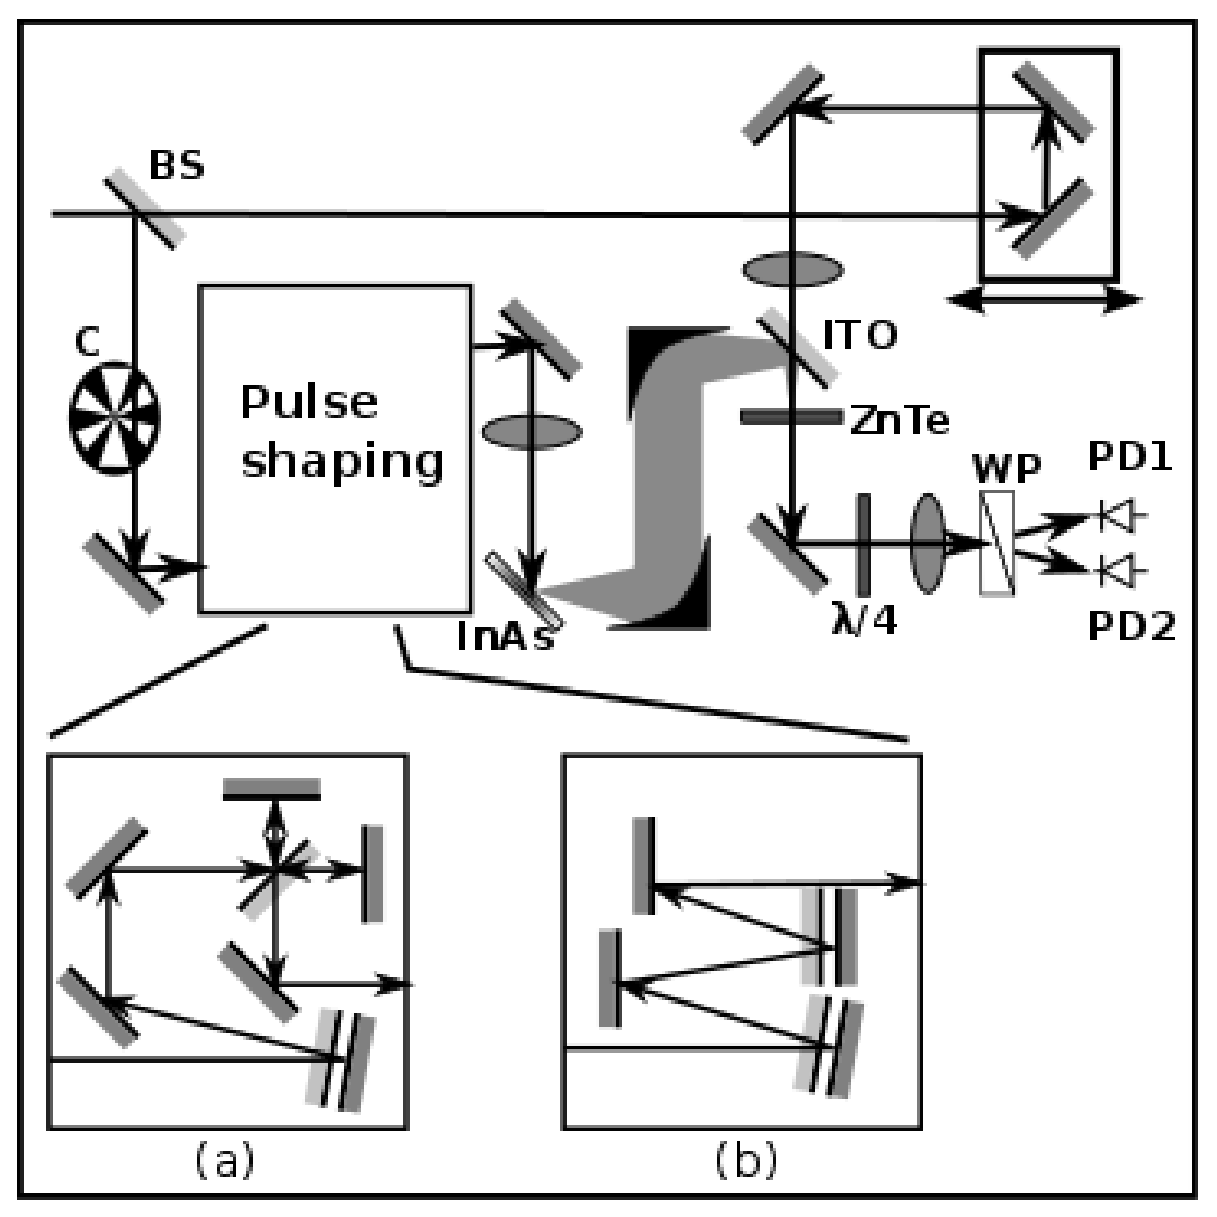
\includegraphics[scale = 0.35]{./Figure1.eps}
  \captionof{figure}{\textcolor{violet}{Schematic of the THz generation
      and detection setup. Two different pulse shaping techniques for
      the optical driving pulse are compared: (a) an etalon followed
      by a Michelson interferometer and (b) two etalons. {\bf BS}:
      beam splitter. {\bf C}: optical chopper. {\bf InAs}: Indium
      Arsenide semiconductor chip.  {\bf ITO}: Indium Tin Oxide coated
      glass substrate. {\bf ZnTe}: Zinc Telluride detection
      crystal. {\bf $\lambda/4$}: quarter waveplate. {\bf WP}:
      Wollaston prism. {\bf PD1} and {\bf PD2}: Photodiodes used for
      balanced detection.}}
  \label{Fig: Experimental setup}
 \end{minipage}

 \textcolor{BurntOrange}{Figure \ref{Fig: Experimental setup}(a) shows
   the first pulse train generation scheme tested, an etalon followed
   by a Michelson interferometer. The etalon consists of a broadband
   dielectric partial reflector (39\% reflective at normal incidence)
   and a high reflecting silver mirror...}

 \textcolor{Sepia}{Despite this overlap of pulses, we do not expect
   effects from interference between the two copies of the pulse
   train. The fourth pulse in the train has, at most, 10\% of the
   intensity of the first pulse of the copied train. More importantly,
   however, in order to interfere, the two optical pulses must be
   overlapped in time and space to a degree of precision higher than
   required for this pulse train to effectively shape the THz. This is
   a result of the difference in time duration between the optical
   pulses ($\sim$50 fs) and the THz pulses ($\sim$1 ps). In fact, an
   advantage of our pulse shaping method is that we do not require the
   alignment precision and stability required in a interferometric
   scheme...}

 \textcolor{ForestGreen}{The THz radiation is steered and focused,
   using two off-axis, parabolic, gold-coated mirrors, onto a 1-mm
   thick ZnTe crystal for electro-optic detection
   [citation]}. \textcolor{BurntOrange}{ All measurements were
   performed in a nitrogen-purged environment with 3\%-4\% humidity to
   minimize absorption by water.}

\end{em}

A common pitfall when writing the experimental description is to
create a chronological list of the steps that were taken during the
experiment. Avoid this. Describe the setup and the experiment, not
your journey through it.

\textit{\textbf{Schematic drawing tool:}} You must use software to
make the experimental figure. There are two kind of drawing tools:
pixel drawing software and vector drawing software. Vector graphic
software is usually a little harder to learn but produces images that
can scale without running into pixelation issues. Here is list of
possible tools:

\begin{itemize}[label=-]
 \item Vector graphics: Inkscape (our recommendation), RollApp, LibreOffice Draw,
 Adobe Illustrator
 \item Pixel graphics: Krita, LibreOffice Draw, GIMP, Photoshop, PowerPoint
 \item Circuit diagrams: circuitikz, www.circuit-diagram.org, www.circuitlab.com
\end{itemize}

\subsubsection{Computational methods}

The methods section will look significantly different for an article
reporting computational work. In such a paper, the methods section
should include:

\begin{itemize}
\item The math involved to transition the information in the theory
  section into a model. For example, if you are solving a differential
  equation, you should write down how you simplified the equations and
  solved the derivatives in the methods section.
\item Any approximation you made to simplify the equations and make
  them easier or more efficient to solve.
\item The limits of the code in terms of resolution and/or stability.
\item How long it takes to run the code under what conditions.
\item A description of what specific simulation was run. Consider the
  example of simulating free fall. What were the initial velocity and
  position for each simulation?
\end{itemize}

\newpage

\subsection{Data and analysis}
\label{sec:Data}

\subsubsection{What to include}

In this section, you use your data to prove your claims. You build
your argument using the ideas you've developed in the theory and
experimental description sections. You are telling a story of
sorts. Think in terms of a narrative, not a step-by-step description
of the math you did.

This section will include:

\begin{itemize}
\item \textcolor{ForestGreen}{properly formatted figures and tables.}
  The format depends on the data being presented. Small data sets
  without a functional dependence can be presented in a table. Long
  data sets, or data sets where we expect a trend, should be presented
  in a graph.
\item a \textcolor{red}{discussion of each graph in the text}. If you
  find that you have nothing to say about a figure, it might be a
  indication that it should not be there.
\item a discussion of the \textcolor{BurntOrange}{uncertainty in the
    results.} This discussion should include the likely sources of
  uncertainty and their effects on the data.
\item a \textcolor{violet}{comparison} between your results and those
  expected from primary sources when those comparisons are available.
\item \textcolor{Sepia}{a discussion of your results and what they
    mean.}
\end{itemize}

Below is an example:

\textcolor{red}{Figure \ref{fig spectrum selectivity} shows the
  detected THz spectra obtained by using our two different pulse
  shaping configurations. In figure \ref{fig spectrum selectivity}(a),
  narrow spectral peaks were observed when using the etalon-Michelson
  interferometer method for pulse shaping (see figure \ref{Fig:
    Experimental setup}(a)). The position of the peak is determined by
  changing the spacing between the partial and high reflector in the
  etalon and the relative lengths of the arms of Michelson
  interferometer. The width of the peak is controlled by the number of
  pulses in the optical train. For comparison, the plot includes the
  broad THz spectrum measured when a single 800 nm pulse is incident
  on the InAs. The relative amplitude of the broadband spectrum to
  that of the narrowband peaks has been amplified for easier
  comparison. In figure \ref{fig spectrum selectivity}(b), the 800 nm
  laser pulse was shaped using two etalons (see figure \ref{Fig:
    Experimental setup}(b)). The normalized broadband spectrum from a
  single driving pulse is also shown for reference. The differences in
  shape of the broad spectra shown in figure \ref{fig spectrum
    selectivity} are typical of day-to-day variations in humidity and
  alignment.}

\begin{minipage}{\linewidth}
 \centering
 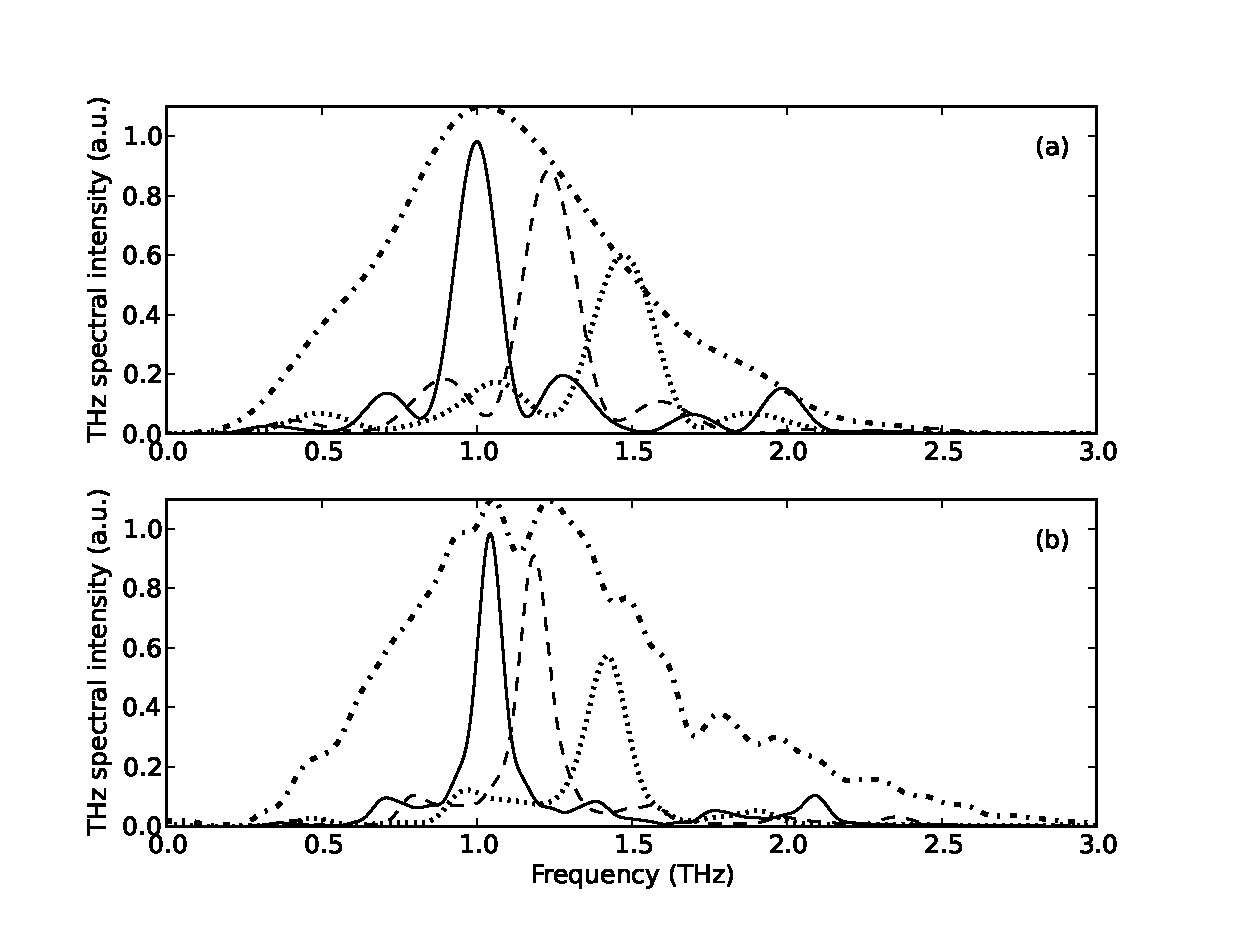
\includegraphics[scale = 0.5]{./Figure2.eps}
 \captionof{figure}{\textcolor{ForestGreen}{Data showing frequency
     selection for (a) the etalon followed by a Michelson
     interferometer pulse shaping configuration and (b) two
     consecutive etalons. The peaks displayed in (a) are centered at
     0.99 THz, 1.22 THz, and 1.47 THz. The peaks in (b) are centered
     at 1.03 THz, 1.18 THz, and 1.41 THz. For both figures, the broad
     spectrum of the THz pulse arising from a single shaped 800 nm
     laser pulse is also shown.}}
 \label{fig spectrum selectivity}
\end{minipage}

\textcolor{Sepia}{Comparing the two sets of data in figure \ref{fig
    spectrum selectivity} clearly shows that we obtain better
  frequency selectivity in the case of two etalons compared to one
  etalon and one Michelson interferometer. The peak centered at 1.22
  THz in figure \ref{fig spectrum selectivity}(a) has
  $\Delta f / f = 0.16$ whereas the peak centered at 1.18 THz in
  figure \ref{fig spectrum selectivity}(b) has $\Delta f / f =
  0.10$. This can be readily explained...}
\textcolor{BurntOrange}{Saturation effects in the InAs, however, limit
  the use of simple Fourier transforms to accurately model the
  expected THz spectrum as is discussed later in the text.}

\textcolor{violet}{The high energy throughput and mechanical stability
  of the two-etalon setup is quite favorable compared to other pulse
  shaping schemes. We compare our results to those of Vidal \textit{et
    al.} [CITATIONS] (SLM in the frequency dispersed plane of a zero
  dispersion stretcher) and Chen \textit{et al.} [CITATIONS] (etalon
  after a stretcher) as they are the most efficient methods to
  date. In the first case, ...}

\textcolor{Sepia}{Another advantage of using only etalons for pulse
  shaping is the ease with which the technique can be expanded. A
  pulse shaping scheme using 3 or 4 etalons, for example,...}

\subsubsection{Additional concerns}

\textit{\textbf{Data analysis and visualization software:}} There are many
types of software available to analyze and draw data. The list below splits
the options into Open source and closed source categories. Open source
options are usually free and equally powerful as the closed source versions
but do not have the same polish in the user interface.

\begin{itemize}[label=-]
 \item Open source: Python is our recommendation for plotting, fits, filtering, and most other aspects of your analysis. Other resources include SciDAVis, QtiPlot, and Octave.
 \item Closed source: Origin, Matlab, Mathematica, Igor Pro, etc.
\end{itemize}

\newpage

\subsection{Conclusion}
\label{sec:Conclusion}

Your conclusion should:

\begin{itemize}
\item \textcolor{BurntOrange}{restate} the results of the experiment.
\item not present any new information.
\item \textcolor{violet}{suggest future work.}
\item end with a \textcolor{ForestGreen}{broader view} of your work
  and its significance.
\end{itemize}

Below is an example:

\textcolor{BurntOrange}{In conclusion, we have demonstrated the use of
  two staggered etalons as a high through- put pulse shaping method
  for THz generation. We used an un-biased InAs chip as our THz
  emitter and demonstrated bandwidth selectivity $\Delta$f /f = 0.10
  at 1.18 THz. Carrier satu- ration effects in the InAs were shown to
  add additional pulse shaping to the THz electric field but not to
  prevent high selectivity in bandwidth.} \textcolor{violet}{Our data
  indicate that the system could easily be expanded to include more
  etalons which would result in better frequency selectivity while
  maintaining a high energy efficiency.} \textcolor{ForestGreen}{While
  useful for any laser system, this method is especially well suited
  for low-power laser systems that cannot afford the power loss
  associated with many other pulse shaping techniques and for
  researchers developing applications needing a modular approach.}

\newpage

\subsection{Acknowledgments}
\label{sec:Acknowledgments}

Not all reports need an acknolwedgement section, but it is a standard 
section for scientific articles wherein the authors acknowledge support
from various sources, whether from a genuine sense of gratitude or by
contractual obligation. For example, for a scientific study receiving
funding from a particular government funding agency, private foundation, 
or commercial partner, the sources of funding must always be cited.

\subsubsection{Informal support from people}

In many cases, it is also a good idea to mention people who helped with
the project but who did not meet the criteria
to be included as an official coauthor on the the paper. This could include
people whom the authors asked for advice; people who gave feedback on drafts; and/or 
people who provided materials that enabled the work to occur. Of course, if a person
contributed significant ideas and work to the report itself, they should generally be
listed as a coauthor rather than merely acknowledged at the end. Different scientific
journals and fields have different criteria for coauthorship: for example, the
American Astronomical Society says:

\textit{All persons who have made significant 
contributions to a work intended for publication should be offered the opportunity 
to be listed as authors. This includes all those who have contributed significantly 
to the inception, design, execution, or interpretation of the research to be reported.}

For your reports in this class, only the members of your group should be listed as
``authors'' of the report, but it may be appropriate to mention other classmates or
people who provided ideas, suggestions, or feedback that you took into consideration 
when conducting your experiment or completing your report.

\subsubsection{AI and LLMs}

One essential element to include in your acknowledgements section is any use of 
artificial intelligence (AI) or large-language models (LLMs). These tools are
often used in many different aspects of scientific work including the writing
of analysis code, generation of schematic diagrams, as well as the generation, 
formatting, and editing of text. Most scientific journals have policies governing
the acceptable use of AI in production of scientific studies.

For our course, using AI tools is allowed to help you make sure your analysis code
is working properly, and it may also be used to help you with grammar and formatting.
Any such use of AI should be described explicitly in the acknowledgement section of 
your paper (i.e., you should describe what parts of the analysis, writing, formatting,
etc. you used these tools for and how you used them).

AI tools should \textit{not} be used to generate text wholesale to be copied into
your lab report: e.g., it should not be used to generate an introduction or a derivation 
that you include directly. Likewise, you should not use AI tools to generate code that you 
do not understand, as it may give erroneous results. At every stage, make sure
that your submitted report reflects your own work and your own understanding of your
results and their context.


\newpage

\subsection{References}
\label{sec:References}

References should appear at the end of the report and be formatted as:\\

- Names, {\it Title}, Publication, Date\\

Below are examples of {\it when} to use citations in your report.

In the introduction, use citations...

\begin{itemize}
\item to flesh out the broader context of your research.
\item to highlight interest in the kind of research you are
  presenting.
\item to point out past results relevant to your claim.
\end{itemize}

In the theory section, use citations to refer to long derivations
you do not have room for in your report (where only a few of the steps
should be shown) and background information that you assume the reader
should be aware of but might still want to refresh on.

In the experimental description section, use citations...

\begin{itemize}
\item to show examples of similar experiment designs.
\item to refer to more complicated experimental techniques that you
  employed in your work.
\end{itemize}

In the data and analysis section, use citations to compare your
results to accepted values or similar measurements.

It is appropriate for a reference to be cited more than once in the
report.  For example, an article cited in the introduction about prior
work done on your topic can be cited again in the analysis if you are
comparing your results to those presented in the article.


\newpage

\section{Checklist: After you write}
\label{sec:post-chk}

\begin{todolist}

\item Review every single sentence. For each sentence, determine
  whether or not it is needed. What is its purpose? Remove all
  unnecessary sentences.
\item {\bf Verb tense}. The work you did in the lab should be
  described in the past tense. Your results and conclusions should be
  written in the present tense since they are (hopefully) still valid.
\item {\bf Voice}. You should write in the active voice. For example,
  don't write:

  \begin{em}
    \textcolor{red}{The data were taken...}
  \end{em}

  You can always tell that a sentence is written in the passive voice
  if you can add ``... by vampires'' at the end. Instead, write:

  \begin{em}
    \textcolor{ForestGreen}{We used the apparatus to measure...}
  \end{em}
\item Check your report for informal and/or imprecise language. Don't
  write:

  \begin{em}
    \textcolor{red}{We saw pretty good agreement between the theory
      and our experiment.}
  \end{em}

  Instead, write:

  \begin{em}
    \textcolor{ForestGreen}{The accepted value for the speed of sound
      in the lab is 343 m/s. We measured (335$\pm$10) m/s.}
  \end{em}

  Don't write:

  \begin{em}
    \textcolor{red}{We had to keep a careful eye on the temperature
      gauge to make sure things worked okay.}
  \end{em}

  The assumption is that you did everything carefully. Instead, write:

  \begin{em}
    \textcolor{ForestGreen}{We monitored the temperature during the
      experiment.}
  \end{em}

\item Check the style guide.
\item Put the paper down for at least half a day. Then re-read it with
  a fresh mind.
\item If there is time, have a another student read the report.
\item If there is time, read the report to yourself slowly and out
  loud.

\end{todolist}

\newpage

\section{Style guides}
\label{sec:style}

When publishing a manuscript in a scientific journal, there are many
rules to formatting text, figures, etc. These rules are covered in the
style guides for the individual journals. In this course, we use the
following rules:

% \rule{\textwidth}{0.5pt}

\subsection{Figures and Tables}
\begin{itemize}
\item {{\bf All tables and figures must be mentioned explicitly by
      number} and appear in the correct numerical order.  That is,
    Tables 1, 2, 3, and 4 must each be mentioned in the text at least
    once, and the first mention of Table 3 should not precede the
    first mention of Table 2. \par}

  {\footnotesize \sf Note: Don't directly type the number of any table or
    figure; have latex keep track of the numbers using \verb+\label+
    and \verb+\ref+.  See examples in templates.\par}
\end{itemize}

\subsubsection{Figures}

\begin{itemize}
\item {\bf All figures must have a caption} and figure captions should
  clearly and concisely label and explain figures and parts of
  figures. The first sentence of each figure caption should be a
  descriptive phrase, omitting the initial article (the, a, an).

\item {\bf In multi-part figures, the captions should distinguish (a),
    (b), (c), etc., components of the figure.} Note that if parts are
  identified in the legend as (a), (b), (c), particularly for single
  figures composed of multiple panels, these letters should be clearly
  labeled in the figure itself. Otherwise panels should be referred to
  by position (top right, top left, middle, bottom, etc.)

\item {\bf All lines} (solid, dashed, dot-dashed, dash-dotted, etc.)
  {\bf and symbols} (filled or open circles, squares, triangles,
  crosses, arrows, etc.) {\bf should be explained in the caption.}

\end{itemize}

\subsubsection{Tables}

\begin{itemize}
\item {\bf Every table must have a caption} and the caption should be
  a concise title (less than a sentence); more extensive descriptions
  or secondary information should be incorporated in a note to the
  table.

\item {\bf Each column, including the first, must have a heading.}
  Column headings should label the entries concisely (one or two
  words); the first letter of each word is capitalized.

\item {\bf Units of measurement should be given in parentheses
    immediately below the column headings}, not listed with the data
  in the body of the table.

\end{itemize}

\subsection{Equations}

\begin{itemize}
\item {{\bf Equations should not be referred to by their numbers
      alone}; that is, say ``substituting in Eq.~(45)'' rather than
    ``substituting in (45).'' \par}

  {\footnotesize \sf Note: Don't directly type the number of any equation;
    have latex keep track of the numbers using \verb+\label+ and
    \verb+\ref+.\par}

\item {\bf Values given in scientific notation should be expressed
    with a multiplication sign} preceding the power of 10 (e.g.,
  $3.4\times10^{-18}$); in tables only, to conserve space, the form
  3.4E-18 may be used.

\item {\bf Stacked fractions are not permitted in the body of the text
    or in superscripts}: that is, inline and superscript fractions
  should be set as $dt /ds$, not $\frac{dt}{ds}$.
\end{itemize}

\subsection{Miscellaneous}

\begin{itemize}

\item {\bf Acronyms and abbreviations should be spelled out the first
    time they are used} unless they are common throughout the
  discipline. Terms defined in the abstract should be defined
  independently in the main text.

\item {\bf Symbols for chemical elements are in normal type}, not
  italics. The mass number precedes the symbol (e.g., $^{12}$C).

\item {\bf Use standard abbreviations for SI} (e.g., m, km, mm) {\bf
    and natural units} (e.g., au, pc, cm). If English units such as
  inches or pounds per square inch are used, metric equivalents should
  follow in parentheses.

\item {\bf Avoid beginning sentences with a symbol, number, or
    lower-case letter.}

\item {\bf The word ``data'' is plural and takes a plural verb (i.e. ``these data are displayed in Fig. 2'' rather than ``this data is displayed in Fig. 2'').}

\end{itemize}

\end{document}
